\documentclass[11pt]{article}
\usepackage{amsmath, amssymb, amsthm, bbm}
\usepackage{graphicx}
\usepackage{hyperref}
\usepackage{tikz, subcaption}
\usepackage{enumitem}
\usepackage{geometry}
\usepackage{algorithm}
\usepackage{algpseudocode}
\usepackage[backend=biber,
    maxnames=10,
    minnames=1,
style=alphabetic]{biblatex}
\addbibresource{references.bib}
\geometry{margin=1in}

\newtheorem{proposition}{Proposition}
\newtheorem{theorem}{Theorem}
\newtheorem{lemma}{Lemma}
\newtheorem{corollary}{Corollary}

\title{Optimization of Graph Squares}
\author{Eddie Xu\\\small\texttt{eddie.xu@student.unimelb.com.au}}
\date{\today}


\begin{document}

\maketitle

\begin{abstract}
In this paper, we investigate the matrix properties of graph squares, focusing in particular on the
relationship between the adjacency matrix of a graph and the corresponding adjacency of its square. 
\end{abstract}

\tableofcontents

\section{Introduction} \label{sec::intro}

The problem of finding the square root of a graph is a well-studied field in both mathematics and computer-science, 
with specific relation to distributed computing, network design and computational biology. Research in this area has
primarily focused around the undirected graph $H$ and its square $G = H^2$ which is obtained by adding an edge between 
every pair of vertices whose distance in $H$ is at most two. 

Much of the existing research on graph square roots has centered on characterizing when a graph admits such 
a root and on the complexity of reconstructing $H$ from $G$. In contrast rather than studying the construction problem 
directly, we analyze the relationship between the adjacency matrix $A_H$ of the root and the adjacency matrix $A_G$ of 
the square, and show that the problem can be completely categorized as an integer program. 

We then examine the 

\section{Background} \label{sec::background}
Let $H = (V, E_H)$ be the undirected \emph{graph root} with $|V|=n$ vertices, and let $G = (V, E_G)$ be the undirected 
\emph{graph square} where the relationship between root $H$ and square $G$ is denoted as $G = H^2$. The
\emph{adjacency matrix} of $G$ can be represented as $A_G$ where edge $ij \in E_G$ exists if and only if $i \neq j$ and 
there is a path in $H$ of length $1$ or $2$ from $i$ to $j$. Equivalently, 
\[
(A_G)_{ij} =
\begin{cases}
1 ,& \text{if } \big( (A_H)_{ij} = 1 \;\text{or}\; (A_H^2)_{ij} > 0 \big) \; \text{for} \; i \neq j, \\
0 ,& \text{otherwise}.
\end{cases}
\]

This definition follows strictly from $(A_H^2)_{ij}$ giving the number of paths of length two between 
vertices $i, j$ and with the \emph{degree matrix} $(D_H)_{ii} = \deg_H(i)$ such that 
\[
A_{G = H^2} = \frac{(A_H)^2 - D_H}{\# \; \text{paths between} \; i, j} + A_H. 
\]
Let $\mathbbm{1}_{\geq 1} : \mathbb{R}^{n \times n} \to \{0,1\}^{n \times n}$ denote the entrywise \emph{indicator function}, defined by
\[
\mathbbm{1}_{\geq 1}(M)_{ij} =
\begin{cases}
1 & \text{if } M_{ij} \geq 1, \\
0 & \text{if } M_{ij} = 0.
\end{cases}
\]
Then the adjacency matrix of the graph square $G$ is given by 
\begin{equation} \label{eq::fund_adj_eq_undirected}
    A_G = \mathbbm{1}_{\geq 1}\!\big((A_H)^2 - D_H + A_H\big).
\end{equation}

\subsection{Integer Program} \label{subsec::IP}
Let $x_{ij} \in \{0, 1\}$ be the decision variables of $A_H$, let $y_{ikj} \in \{0, 1\}$ be the decision variable for 
$x_{ik}x_{kj}$ in $(A_H)^2_{ij}$ and let $z_{ij} \in \mathbb{Z}_{\geq 0}$ represent the argument inside the indicator function. 

$\displaystyle 
D_H =
\begin{bmatrix}
\deg_H(1) & 0      & \cdots & 0 & 0      \\
0         & \ddots & \vdots & \ddots & \vdots \\
\vdots    & \cdots & \deg_H(i) & \cdots & 0      \\
0         & \ddots & \vdots & \ddots & \vdots \\
0         & \cdots & 0      & \cdots & \deg_H(n)
\end{bmatrix}, 
$ 
$\displaystyle A_H =
\begin{bmatrix}
x_{11} & \cdots & x_{1j} & \cdots & x_{1n} \\
\vdots  & \ddots  & \vdots & \ddots & \vdots  \\
x_{i1} & \cdots & x_{ij} & \cdots & x_{in} \\
\vdots  & \ddots  & \vdots & \ddots & \vdots  \\
x_{n1} & \cdots & x_{nj} & \cdots & x_{nn}
\end{bmatrix}
$ such that 
\[
(A_H)^2 = \begin{bmatrix}
\displaystyle \sum_{k=1}^n x_{1k}x_{k1} & \cdots & \displaystyle \sum_{k=1}^n x_{1k}x_{kj} & \cdots & \displaystyle \sum_{k=1}^n x_{1k}x_{kn} \\
\vdots  & \ddots  & \vdots & \ddots & \vdots  \\
\displaystyle \sum_{k=1}^n x_{ik}x_{k1} & \cdots & \displaystyle \sum_{k=1}^n x_{ik}x_{kj} & \cdots & \displaystyle \sum_{k=1}^n x_{ik}x_{kn} \\
\vdots  & \ddots  & \vdots & \ddots & \vdots  \\
\displaystyle \sum_{k=1}^n x_{nk}x_{k1} & \cdots & \displaystyle \sum_{k=1}^n x_{nk}x_{kj} & \cdots & \displaystyle \sum_{k=1}^n x_{nk}x_{kn}
\end{bmatrix}.
\]
Then with known constants $g_{ij} \in \{0, 1\}$ from $A_G$, can reformulating \eqref{eq::fund_adj_eq_undirected} as an 
integer program by equating entries of each matrix to give the following linear system of $n^2$ equations.
\begin{equation}  \label{eq::fund_programming_equation}
\begin{bmatrix}
g_{11} \\
\vdots \\
g_{1j} \\
\vdots \\
g_{1n} \\
\vdots \\
g_{ij} \\
\vdots \\
g_{nn}
\end{bmatrix} 
=
\begin{bmatrix}
\mathbbm{1}_{\geq 1}\big(z_{11}\big) \\
\vdots \\
\mathbbm{1}_{\geq 1}\big(z_{1j}\big) \\
\vdots \\
\mathbbm{1}_{\geq 1}\big(z_{1n}\big) \\
\vdots \\
\mathbbm{1}_{\geq 1}\big(z_{ij}\big) \\
\vdots \\
\mathbbm{1}_{\geq 1}\big(z_{nn}\big)
\end{bmatrix}
=
\begin{bmatrix} \displaystyle
\mathbbm{1}_{\geq 1}\!\big(\sum_{k=1}^n x_{1k}x_{k1} - (D_H)_{11} + x_{11} \big) \\
\vdots \\ \displaystyle
\mathbbm{1}_{\geq 1}\!\big(\sum_{k=1}^n x_{1k}x_{kj} - (D_H)_{1j} + x_{1j} \big) \\
\vdots \\ \displaystyle
\mathbbm{1}_{\geq 1}\!\big(\sum_{k=1}^n x_{1k}x_{kn} - (D_H)_{1n} + x_{1n} \big)\\
\vdots \\ \displaystyle
\mathbbm{1}_{\geq 1}\!\big(\sum_{k=1}^n x_{ik}x_{kj} - (D_H)_{ij} + x_{ij} \big)\\
\vdots \\ \displaystyle
\mathbbm{1}_{\geq 1}\!\big(\sum_{k=1}^n x_{nk}x_{kn} - (D_H)_{nn} + x_{nn} \big)
\end{bmatrix}.
\end{equation}
The matrix $D_H$ is diagonal can be represented as $\displaystyle (D_H)_{ii} = \sum_{k} x_{ik}$ where $(D_H)_{ij} = 0$ for $i \neq j$. 
Let $M \in \mathbb{Z}_{> 0}$ be a sufficiently large constant. The known 
$z_{ij}$ represent the terms inside the indicator function such that
\[
g_{ij} = 1 \iff z_{ij} \geq 1 \;\text{and}\; g_{ij} = 0 \iff z_{ij} = 0.
\] The above condition can be modelled using a standard big-$M$ formulation,
and the resulting integer program is given by
\begin{alignat}{3}
\text{Variables: } & \nonumber \\ 
& x_{ij} \in \mathbb{Z}_{\geq 0}, 
&& \forall i,j \in \{1, \dots, n\}, \label{eq::IP_x_variable} \\ 
& y_{ikj} \in \mathbb{Z}_{\geq 0}, 
&& \forall i,k,j \in \{1, \dots, n\}, \label{eq::IP_y_variable} \\
& z_{ij} \in \mathbb{Z}_{\geq 0}, 
&& \forall i,j \in \{1, \dots, n\}. \label{eq::IP_z_variable} \\
\text{Constraints: } & \nonumber \\
\text{(1) Indicator argument: } 
& z_{ii} = \sum_{k = 1}^{n}y_{iki} - \sum_{k = 1}^{n} x_{ik} + x_{ii}, 
&& \forall i \in \{1, \dots, n\} , \label{eq::IP_fund_matrix} \\
& z_{ij} = \sum_{k = 1}^{n}y_{ikj} + x_{ij}, 
&& \forall i \neq j \in \{1, \dots, n\} , \label{eq::IP_indicator_arg} \\
\text{(2) Indicator function: } 
& z_{ij} \leq M g_{ij}, 
&& \forall i, j \in \{1, \dots, n\}, \label{eq::IP_indicator_upper} \\
& z_{ij} \geq g_{ij}, 
&& \forall i, j \in \{1, \dots, n\}, \label{eq::IP_indicator_lower}\\
\text{(3) Product: } 
& y_{ikj} \leq x_{ik}, 
&& \forall i, k, j \in \{1, \dots, n\}, \label{eq::IP_product_upper_first} \\
& y_{ikj} \leq x_{kj}, 
&& \forall i, k, j \in \{1, \dots, n\}, \label{eq::IP_product_upper_second} \\
& y_{ikj} \geq x_{ik} + x_{kj} - 1, 
&& \forall i, k, j \in \{1, \dots, n\} \label{eq::IP_product_lower} \\
\text{(4) Upper Bound: } 
& x_{ij} \leq 1, 
&& \forall i, j \in \{1, \dots, n\}, \label{eq::IP_x_upper_bound} \\
& y_{ikj} \leq 1, 
&& \forall i, k, j \in \{1, \dots, n\}, \label{eq::IP_y_upper_bound}. 
\end{alignat} \label{eq::integer_program}

In addition, the adjacency matrix $x$ must satisfy further constraints arising from symmetry and diagonality. Although analogous 
constraints could also be imposed on the auxiliary variables $z$ they are omitted due to redundancy and potentially
introduces artificial degeneracy in the linear program. 
\begin{alignat}{3} 
\text{(5) Symmetry: } 
& x_{ij} = x_{ji}, 
&&\qquad \forall i,j \in \{1, \dots, n\}, \label{eq::IP_symmetry_x} \\
\text{(6) Diagonal: } 
& x_{ii} = 0, 
&&\qquad \forall i \in \{1, \dots, n\}.  \label{eq::IP_diagonal_x} 
\end{alignat}

\subsection{Linear Program} \label{subsec::LP}

The linear relaxation of the integer program defined by Equations~\eqref{eq::IP_x_variable}--\eqref{eq::IP_diagonal_x} is 
constructed in order to generate a feasible weighted solution in polynomial time algorithm. It is done with identical constraints,
however the decision variables \eqref{eq::IP_x_variable}, \eqref{eq::IP_y_variable} and \eqref{eq::IP_z_variable}
are replaced with
\begin{alignat}{3}
& x_{ij} \in  \mathbb{R}_{\geq 0}, 
&&\qquad \forall i,j \in \{1, \dots, n\}, \label{eq::LP_x_variable} \\
& y_{ikj} \in \mathbb{R}_{\geq 0}, 
&&\qquad \forall i,k,j \in \{1, \dots, n\}, \label{eq::LP_y_variable} \\
& z_{ij} \in \mathbb{R}_{\geq 0}, 
&&\qquad \forall i,j \in \{1, \dots, n\} \label{eq::LP_z_variable}. 
\end{alignat} 

The results from the linear programming can give \emph{integer solutions} and \emph{fractional solutions} when the root exists 
and \emph{fractional solutions} and \emph{infeasible solutions} when the root does not exist such that the results in 
Figure~\ref{fig:linear_program_diagram} can be generated. 

\section{Linear Program} \label{sec::LP}
\subsection{Max Objective Function} \label{subsubsec::max_obj}

Consider the addition of an objective function maximizing the total weights on all edges to the linear relaxation 
defined by Equations~\eqref{eq::IP_fund_matrix}--\eqref{eq::LP_z_variable} in Section~\ref{subsec::LP} 
\begin{equation} \label{eq::max_obj_function}
  \max \sum_{i=1}^{n} \sum_{j=1}^{n} x_{ij}.
\end{equation}

This addition gives the improved results in Figure~\ref{fig:max_objective_function_diagram}.

\subsection{Singular Triangular Decomposition} \label{subsubsec::singular_triangular_decomposition}

Using the local triangular structure of the graph, certain edge assignments in a square root can be fixed. 
For a vertex $s \in V$, define
\[
T(s) = \bigl\{ \{u,v\} \subseteq V \setminus \{s\} \; \vert \;
(s,u)\in E,\ (s,v)\in E,\ (u,v)\in E
\bigr\}
\]
to be the set of triangles in $G$ that contain $s$. If $|T(s)| = 1$ where $T(s) = \{\{u,v\}\}$ then the vertex $s$ 
exists in a unique triangle of $G$. When the neighbours are structurally distinct with different degree 
$\deg_G(u) \neq \deg_G(v)$, then the vertex with smaller degree must be the leaf-adjacent vertex in the square root.  
We enforce the deterministic assignment
\begin{equation}
x_{s w} = 1, \; x_{w s} = 1 \text{ where } 
w=\arg\min\{\deg_G(u), \deg_G(v)\}.
\label{eq:singular_triangle_fix}
\end{equation}

If $\deg_G(u) = \deg_G(v)$, no constraint is imposed. This addition gives the improved results in 
Figure~\ref{fig:singular_triangular_decomposition_diagram} whilst maintaining polynomial runtime. 

In the case of $\deg_G(u) = \deg_G(v)$, enforcement is done by arbitrarily choosing one of the edges of only one 
such triangle. This is done recursively until all such singular triangles are resolved. This gives the improved 
results in Figure~\ref{fig:recursive_singular_triangular_decomposition_diagram}.  

Ross and Harary in 1960 gave an algorithm for constructing a tree root by using characterizations of the square graph 
to conclude that existing tree square roots are unique up to isomorphism \cite{ross_1960_square}.

\begin{proposition}
  Singular triangular decomposition completely categorizes all triangle roots in polynomial time linear program. 
\end{proposition}

% \subsubsection{Tree Constraint} \label{subsubsec::tree_constraint}

% Ross and Harary in 1960 gave an algorithm for constructing a tree root by using characterizations of the square graph 
% to conclude that existing tree square roots are unique up to isomorphism \cite{ross_1960_square}. We investigate whether
% the linear program constrained to only tree square roots can likewise solve the problem in polynomial time. 

% Consider the addition of the following constraints which enforce $n-1$ edges and no cycles for every subset of $V$. 
% \begin{alignat}{3}
% & \sum_{i = 1}^n \sum_{j = 1}^n x_{ij} = 2(n - 1), 
% && \label{eq::spanning_tre} \\
% & \sum_{i \in S} \sum_{j \in S} x_{ij} \le |S| - 1,
% && \forall S \subseteq \{1,\dots,n\},\ |S|\ge 2 \label{eq::subset_cycles}. 
% \end{alignat} 

% NOT POSSIBLE since $x_{ij}$ MUST be fractional and not integer. 

\subsection{Rounding} \label{subsubsec:rounding}

LP fractional solutions are derived from the LP when the root $H$ exists and does not exist. An attempt for rounding 
is achieved such that the classification in Figure~\ref{fig:rounding_max_objective_function_diagram} is obtained.   


\subsection{Dual Problem} \label{subsec::dual_prob} 

We now consider the dual formulation of the max objective linear program defined in Section~\ref{subsubsec::max_obj}
by first restating it in canonical form.

\begin{alignat}{3}
\text{Objective Function: } & \nonumber \\
& \min - \sum_{i=1}^{n} \sum_{j=1}^{n} x_{ij}. \label{eq::primal_max_obj_function}
\end{alignat}
\begin{alignat}{3}
\text{Variables: } & \nonumber \\ 
& x_{ij} \in \mathbb{R}_{\geq 0} \, \Big([0,1]\Big), 
&&\qquad \forall i,j \in \{1, \dots, n\}, \label{eq::standard_LP_x_variable} \\
& y_{ikj} \in \mathbb{R}_{\geq 0} \, \Big([0,1]\Big), 
&&\qquad \forall i,k,j \in \{1, \dots, n\}, \label{eq::standard_LP_y_variable} \\
& z_{ij} \in \mathbb{R}_{\geq 0}, 
&&\qquad \forall i,j \in \{1, \dots, n\} \label{eq::standard_LP_z_variable}. \\
\text{Constraints: } & \nonumber \\
\text{(1) Indicator argument: } 
& z_{ii} - \sum_{k = 1}^{n}y_{iki} + \sum_{k = 1}^{n} x_{ik} - x_{ii} = 0, 
&& \forall i \in \{1, \dots, n\} , \label{eq::standard_IP_fund_matrix} \\
& z_{ij} - \sum_{k = 1}^{n}y_{ikj} - x_{ij} = 0, 
&& \forall i \neq j \in \{1, \dots, n\} , \label{eq::standard_IP_indicator_arg} \\
\text{(2) Indicator function: } 
& z_{ij} - M g_{ij} \leq 0, 
&& \forall i, j \in \{1, \dots, n\}, \label{eq::standard_IP_indicator_upper} \\
& - z_{ij} + g_{ij} \leq 0, 
&& \forall i, j \in \{1, \dots, n\}, \label{eq::standard_IP_indicator_lower}\\
\text{(3) Product: } 
& y_{ikj} - x_{ik} \leq 0, 
&& \forall i, k, j \in \{1, \dots, n\}, \label{eq::standard_IP_product_upper_first} \\
& y_{ikj} - x_{kj} \leq 0, 
&& \forall i, k, j \in \{1, \dots, n\}, \label{eq::standard_IP_product_upper_second} \\
&  x_{ik} + x_{kj} - y_{ikj} - 1 \leq 0, 
&& \forall i, k, j \in \{1, \dots, n\}, \label{eq::standard_IP_product_lower} \\
\text{(4) Symmetry: } 
& x_{ij} - x_{ji} = 0, 
&&\qquad \forall i,j \in \{1, \dots, n\}, \label{eq::standard_IP_symmetry_x} \\
\text{(5) Diagonal: } 
& x_{ii} = 0, 
&&\qquad \forall i \in \{1, \dots, n\}, \label{eq::standard_IP_diagonal_x} \\
\text{(6) Variable Bound: } 
& x_{ij} - 1 \leq 0,
&& \forall i, j \in \{1, \dots, n\}, \label{eq::standard_x_upper_bound} \\
& y_{ikj} - 1 \leq 0,
&& \forall i,k, j \in \{1, \dots, n\} \label{eq::standard_y_upper_bound}.
\end{alignat} \label{eq::linear_program}

This gives the dual problem with 
\begin{alignat}{3}
\text{Objective Function: } & \nonumber \\
\max \quad
&
\sum_{i=1}^n \sum_{j=1}^n
\Bigl(
- M g_{ij}\gamma_{ij}
+ g_{ij}\delta_{ij}
- \lambda_{ij}
\Bigr)
- \sum_{i=1}^n \sum_{k=1}^n \sum_{j=1}^n
\bigl(
\eta_{ikj}
+ \mu_{ikj}
\bigr).
\end{alignat}

\begin{alignat}{3}
\text{Dual Variables: } & \nonumber \\
& \alpha_{i} \in \mathbb{R},
&& \forall i\in \{1,\dots,n\},
&& \text{(associated with \eqref{eq::standard_IP_fund_matrix})}, 
\label{eq::dual_alpha} \\
& \beta_{ij} \in \mathbb{R},
&& \forall i \neq j \in \{1,\dots,n\},
&& \text{(associated with \eqref{eq::standard_IP_indicator_arg})},
\label{eq::dual_beta} \\
& \gamma_{ij} \ge 0,
&& \forall i,j \in \{1,\dots,n\},
&& \text{(associated with \eqref{eq::standard_IP_indicator_upper})},
\label{eq::dual_gamma} \\
& \delta_{ij} \ge 0,
&& \forall i,j \in \{1,\dots,n\},
&& \text{(associated with \eqref{eq::standard_IP_indicator_lower})},
\label{eq::dual_delta} \\
& \epsilon_{ikj} \ge 0,
&& \forall i,k,j \in \{1,\dots,n\},
&& \text{(associated with \eqref{eq::standard_IP_product_upper_first})},
\label{eq::dual_epsilon} \\
& \zeta_{ikj} \ge 0,
&& \forall i,k,j \in \{1,\dots,n\},
&& \text{(associated with \eqref{eq::standard_IP_product_upper_second})},
\label{eq::dual_zeta} \\
& \eta_{ikj} \geq 0,
&& \forall i,k,j \in \{1,\dots,n\},
&& \text{(associated with \eqref{eq::standard_IP_product_lower})}, 
\label{eq::dual_eta} \\
& \theta_{ij} \in \mathbb{R},
&& \forall i,j \in \{1,\dots,n\},
&& \text{(associated with \eqref{eq::standard_IP_symmetry_x})}, 
\label{eq::dual_theta} \\
& \iota_{i} \in \mathbb{R},
&& \forall i \in \{1,\dots,n\},
&& \text{(associated with \eqref{eq::standard_IP_diagonal_x})},
\label{eq::dual_iota} \\
& \lambda_{ij} \geq 0,
&& \forall i,j \in \{1,\dots,n\},
&& \text{(associated with \eqref{eq::standard_x_upper_bound})},
\label{eq::dual_lambda}  \\
& \mu_{ikj} \geq 0, 
&& \forall i,k,j \in \{1,\dots,n\},
&& \text{(associated with \eqref{eq::standard_y_upper_bound})}.
\label{eq::dual_mu} 
\end{alignat}
\begin{alignat}{3}
& \text{Dual Constraints: } \nonumber \\
\forall i,j \in & \{1,\dots,n\},
\text{ each primal } x_{ij}: \nonumber \\
&
\begin{cases}
\displaystyle
-1
- \sum_{k=1}^n \epsilon_{iik}
- \sum_{k=1}^n \zeta_{kii}
+ \sum_{k=1}^n \eta_{iik}
+ \sum_{k=1}^n \eta_{kii}
+ \iota_i
+ \lambda_{ii}
\;\ge\; 0,
& \text{if } j=i, \\
\displaystyle
-1
+ \alpha_i
- \beta_{ij}
- \sum_{k=1}^n \epsilon_{ikj}
- \sum_{k=1}^n \zeta_{kij}
+ \sum_{k=1}^n \eta_{ikj}
+ \sum_{k=1}^n \eta_{kij}
+ \theta_{ij}
- \theta_{ji}
+ \lambda_{ij}
\;\ge\; 0,
& \text{if } j\neq i ,
\end{cases}
\label{eq:dual_x_constraints}
\\[1.4em]
\forall i,k,j \in & \{1,\dots,n\},
\text{ each primal } y_{ikj}: \nonumber \\
&
\begin{cases}
\displaystyle
- \alpha_i
+ \epsilon_{iki}
+ \zeta_{iki}
- \eta_{iki}
+ \mu_{iki}
\;\ge\; 0,
& \text{if } j=i, \\
\displaystyle
- \beta_{ij}
+ \epsilon_{ikj}
+ \zeta_{ikj}
- \eta_{ikj}
+ \mu_{ikj}
\;\ge\; 0,
& \text{if } j\neq i ,
\end{cases}
\label{eq:dual_y_constraints}
\\[1.4em]
\forall i,j \in & \{1,\dots,n\},
\text{ each primal } z_{ij}: \nonumber \\
&
\begin{cases}
\displaystyle
\alpha_i
+ \gamma_{ii}
- \delta_{ii}
= 0,
& \text{if } j=i, \\
\displaystyle
\beta_{ij}
+ \gamma_{ij}
- \delta_{ij}
= 0,
& \text{if } j\neq i .
\end{cases}
\label{eq:dual_z_constraints}
\end{alignat}

whereby the Lagrangian is 
\[
\begin{aligned}
\mathcal{L}(x,y,z)
&=
- \sum_{i=1}^n \sum_{j=1}^n x_{ij} + \sum_{i=1}^n \alpha_i
\Bigl(
z_{ii} - \sum_{k=1}^n y_{iki} + \sum_{k=1}^n x_{ik} - x_{ii}
\Bigr)
+ \sum_{i \neq j} \beta_{ij}
\Bigl(
z_{ij} - \sum_{k=1}^n y_{ikj} - x_{ij}
\Bigr) \\
& \quad
+ \sum_{i=1}^n \sum_{j=1}^n
\gamma_{ij}(z_{ij}-Mg_{ij}) 
+ \sum_{i=1}^n \sum_{j=1}^n
\delta_{ij}(-z_{ij}+g_{ij}) 
+ \sum_{i=1}^n \sum_{k=1}^n \sum_{j=1}^n
\epsilon_{ikj}(y_{ikj}-x_{ik}) \\
&\quad
+ \sum_{i=1}^n \sum_{k=1}^n \sum_{j=1}^n
\zeta_{ikj}(y_{ikj}-x_{kj}) 
+ \sum_{i=1}^n \sum_{k=1}^n \sum_{j=1}^n
\eta_{ikj}(x_{ik}+x_{kj}-y_{ikj}-1) \\
&\quad
+ \sum_{i=1}^n \sum_{j=1}^n
\theta_{ij}(x_{ij} - x_{ji})
+ \sum_{i=1}^n 
\iota_{i}x_{ii} 
+ \sum_{i=1}^n \sum_{j=1}^n
\lambda_{ij}(x_{ij}-1)
+ \sum_{i=1}^n \sum_{k=1}^n \sum_{j=1}^n
\mu_{ikj}(y_{ikj}-1).
\end{aligned}
\]
Collecting terms gives
\[
\begin{aligned}
\mathcal{L}(x,y,z)
&=
\sum_{i=1}^n \sum_{j=1}^n
x_{ij}
\Biggl[
-1
+ \mathbf{1}_{\{j=i\}}
\Bigl(
\alpha_i
- \sum_{k=1}^n \epsilon_{ik i}
- \sum_{k=1}^n \zeta_{k i i}
+ \sum_{k=1}^n \eta_{ik i}
+ \sum_{k=1}^n \eta_{k i i}
+ \iota_i
+ \lambda_{ii}
\Bigr)
\\
&\qquad
+ \mathbf{1}_{\{j\neq i\}}
\Bigl(
\alpha_i
- \beta_{ij}
- \sum_{k=1}^n \epsilon_{ikj}
- \sum_{k=1}^n \zeta_{kij}
+ \sum_{k=1}^n \eta_{ikj}
+ \sum_{k=1}^n \eta_{kij}
+ \lambda_{ij}
\Bigr)
+ \theta_{ij} - \theta_{ji}
\Biggr]
\\
&\quad
+ \sum_{i=1}^n \sum_{k=1}^n \sum_{j=1}^n
y_{ikj}
\Biggl[
- \mathbf{1}_{\{j=i\}}\,\alpha_i
- \mathbf{1}_{\{j\neq i\}}\,\beta_{ij}
+ \epsilon_{ikj}
+ \zeta_{ikj}
- \eta_{ikj}
+ \mu_{ikj}
\Biggr]
\\
&\quad
+ \sum_{i=1}^n \sum_{j=1}^n
z_{ij}
\Biggl[
\mathbf{1}_{\{j=i\}}\,\alpha_i
+ \mathbf{1}_{\{j\neq i\}}\,\beta_{ij}
+ \gamma_{ij}
- \delta_{ij}
\Biggr]
\\
&\quad
- \sum_{i=1}^n \sum_{j=1}^n
M g_{ij}\gamma_{ij}
+ \sum_{i=1}^n \sum_{j=1}^n
g_{ij}\delta_{ij}
- \sum_{i=1}^n \sum_{k=1}^n \sum_{j=1}^n
\eta_{ikj}
- \sum_{i=1}^n \sum_{j=1}^n
\lambda_{ij}
- \sum_{i=1}^n \sum_{k=1}^n \sum_{j=1}^n
\mu_{ikj}.
\end{aligned}
\]

This dual formulation 

\appendix

\newpage 

\section{Result Diagrams}
\subsection{Linear Program}

\begin{figure}[!htbp]
\centering
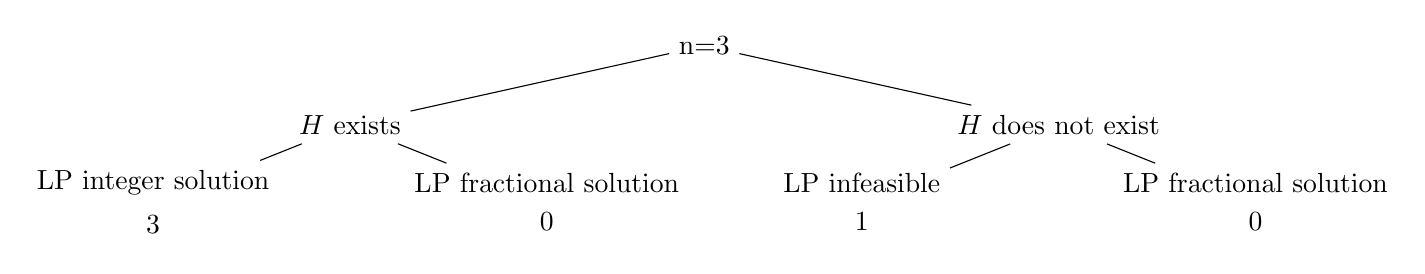
\begin{tikzpicture}[level distance=1cm,
  level 1/.style={sibling distance=9cm},
  level 2/.style={sibling distance=5cm}]
  \node {n=3}
    child { node {$H$ exists}
      child { node {$\underset{\raisebox{-0.8em}{3}}{\text{LP integer solution}}$} }
      child { node {$\underset{\raisebox{-0.8em}{0}}{\text{LP fractional solution}}$} }
    }
    child { node {$H$ does not exist}
      child { node {$\underset{\raisebox{-0.8em}{1}}{\text{LP infeasible}}$} }
      child { node {$\underset{\raisebox{-0.8em}{0}}{\text{LP fractional solution}}$} }
    };
\end{tikzpicture}

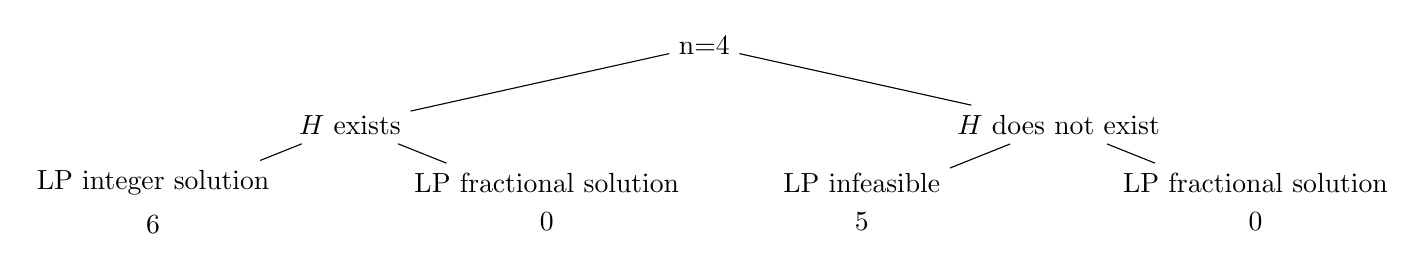
\begin{tikzpicture}[level distance=1cm,
  level 1/.style={sibling distance=9cm},
  level 2/.style={sibling distance=5cm}]
  \node {n=4}
    child { node {$H$ exists}
      child { node {$\underset{\raisebox{-0.8em}{6}}{\text{LP integer solution}}$} }
      child { node {$\underset{\raisebox{-0.8em}{0}}{\text{LP fractional solution}}$} }
    }
    child { node {$H$ does not exist}
      child { node {$\underset{\raisebox{-0.8em}{5}}{\text{LP infeasible}}$} }
      child { node {$\underset{\raisebox{-0.8em}{0}}{\text{LP fractional solution}}$} }
    };
\end{tikzpicture}

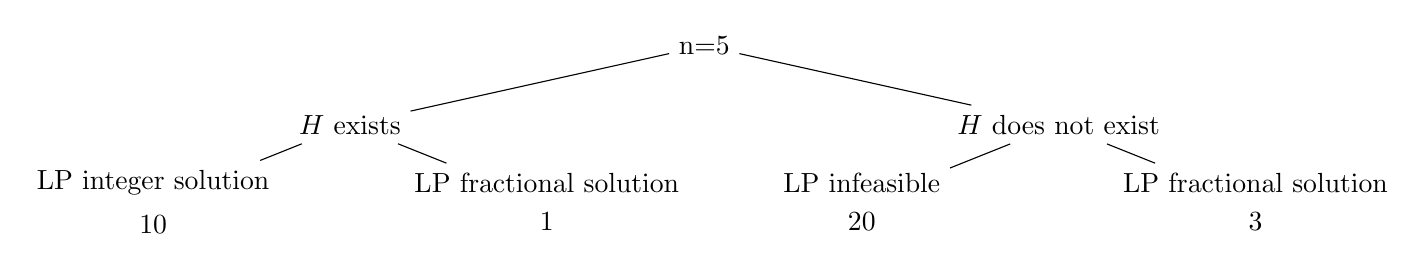
\begin{tikzpicture}[level distance=1cm,
  level 1/.style={sibling distance=9cm},
  level 2/.style={sibling distance=5cm}]
  \node {n=5}
    child { node {$H$ exists}
      child { node {$\underset{\raisebox{-0.8em}{10}}{\text{LP integer solution}}$} }
      child { node {$\underset{\raisebox{-0.8em}{1}}{\text{LP fractional solution}}$} }
    }
    child { node {$H$ does not exist}
      child { node {$\underset{\raisebox{-0.8em}{20}}{\text{LP infeasible}}$} }
      child { node {$\underset{\raisebox{-0.8em}{3}}{\text{LP fractional solution}}$} }
    };
\end{tikzpicture}

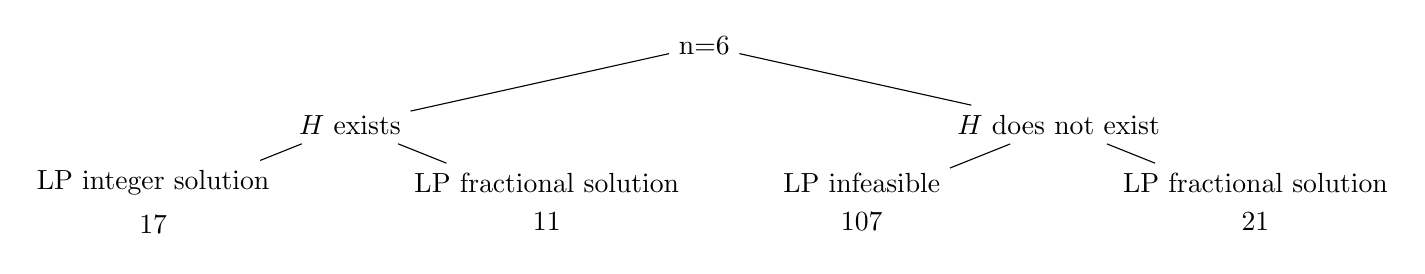
\begin{tikzpicture}[level distance=1cm,
  level 1/.style={sibling distance=9cm},
  level 2/.style={sibling distance=5cm}]
  \node {n=6}
    child { node {$H$ exists}
      child { node {$\underset{\raisebox{-0.8em}{17}}{\text{LP integer solution}}$} }
      child { node {$\underset{\raisebox{-0.8em}{11}}{\text{LP fractional solution}}$} }
    }
    child { node {$H$ does not exist}
      child { node {$\underset{\raisebox{-0.8em}{107}}{\text{LP infeasible}}$} }
      child { node {$\underset{\raisebox{-0.8em}{21}}{\text{LP fractional solution}}$} }
    };
\end{tikzpicture}

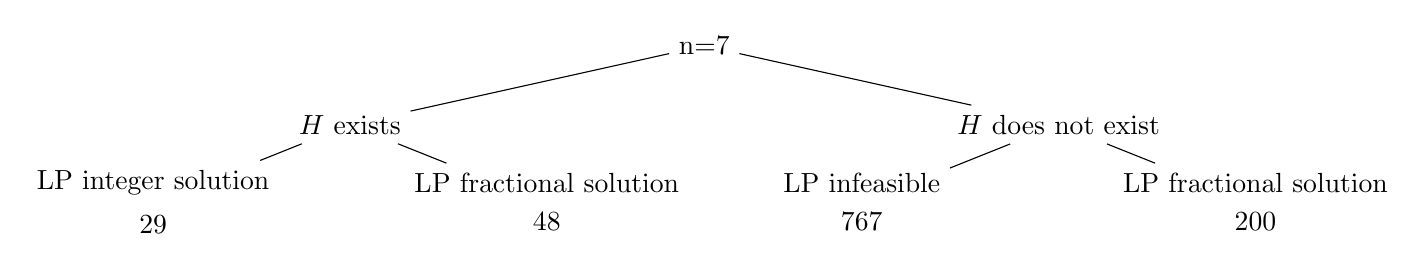
\begin{tikzpicture}[level distance=1cm,
  level 1/.style={sibling distance=9cm},
  level 2/.style={sibling distance=5cm}]
  \node {n=7}
    child { node {$H$ exists}
      child { node {$\underset{\raisebox{-0.8em}{29}}{\text{LP integer solution}}$} }
      child { node {$\underset{\raisebox{-0.8em}{48}}{\text{LP fractional solution}}$} }
    }
    child { node {$H$ does not exist}
      child { node {$\underset{\raisebox{-0.8em}{767}}{\text{LP infeasible}}$} }
      child { node {$\underset{\raisebox{-0.8em}{200}}{\text{LP fractional solution}}$} }
    };
\end{tikzpicture}

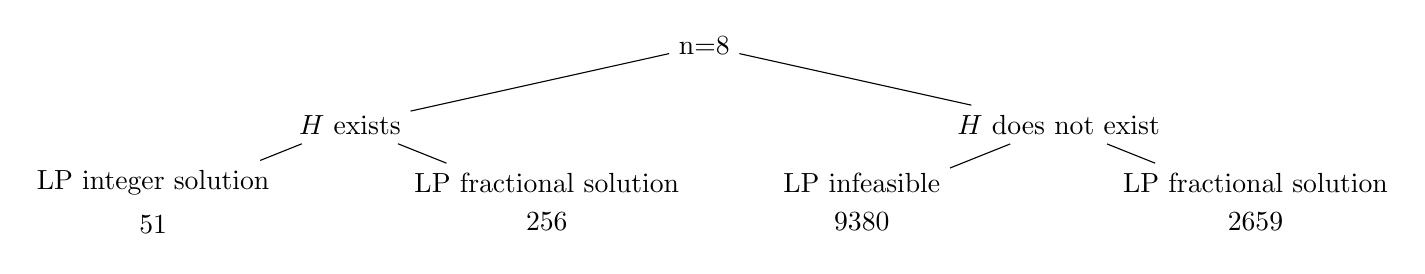
\begin{tikzpicture}[level distance=1cm,
  level 1/.style={sibling distance=9cm},
  level 2/.style={sibling distance=5cm}]
  \node {n=8}
    child { node {$H$ exists}
      child { node {$\underset{\raisebox{-0.8em}{51}}{\text{LP integer solution}}$} }
      child { node {$\underset{\raisebox{-0.8em}{256}}{\text{LP fractional solution}}$} }
    }
    child { node {$H$ does not exist}
      child { node {$\underset{\raisebox{-0.8em}{9380}}{\text{LP infeasible}}$} }
      child { node {$\underset{\raisebox{-0.8em}{2659}}{\text{LP fractional solution}}$} }
    };
\end{tikzpicture}

\caption{LP outcomes for different values of $n$ on base linear program.} 
\footnotemark 
\label{fig:linear_program_diagram} 
\end{figure}

\footnotetext{
The total number of simple graphs on $n=2,3,4,\dots$ unlabeled nodes is the sequence $2, 4, 11, 34, 156, 1044, 12346, \dots$ given by \href{https://oeis.org/A000088}{\texttt{A000088}}. \\
The IP integer solution sequence $2, 3, 6, 10, 17, 29, 51, \dots$ is given by \href{https://oeis.org/A285665}{A285665}. \\
The total number of graphs which are squares is the sequence $2, 3, 6, 11, 28, 77, 307, \dots$ given by \href{https://oeis.org/A382181}{A382181}.}

\newpage

\subsubsection{Max Objective Function}

\begin{figure}[!htbp]
\centering
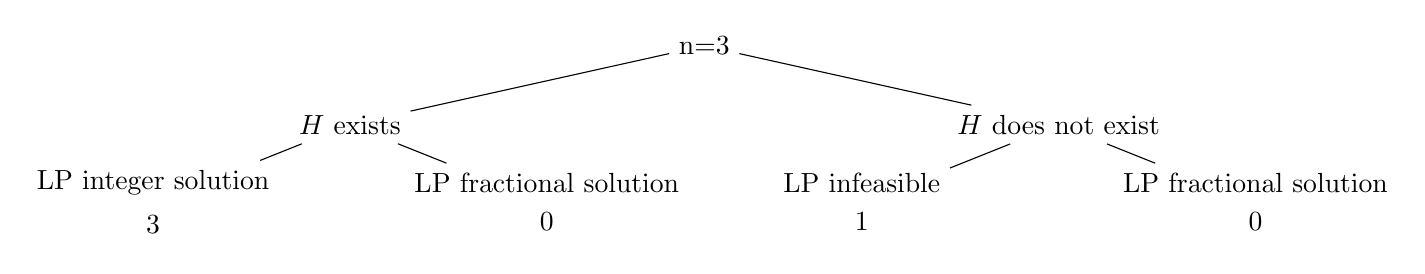
\begin{tikzpicture}[level distance=1cm,
  level 1/.style={sibling distance=9cm},
  level 2/.style={sibling distance=5cm}]
  \node {n=3}
    child { node {$H$ exists}
      child { node {$\underset{\raisebox{-0.8em}{3}}{\text{LP integer solution}}$} }
      child { node {$\underset{\raisebox{-0.8em}{0}}{\text{LP fractional solution}}$} }
    }
    child { node {$H$ does not exist}
      child { node {$\underset{\raisebox{-0.8em}{1}}{\text{LP infeasible}}$} }
      child { node {$\underset{\raisebox{-0.8em}{0}}{\text{LP fractional solution}}$} }
    };
\end{tikzpicture}

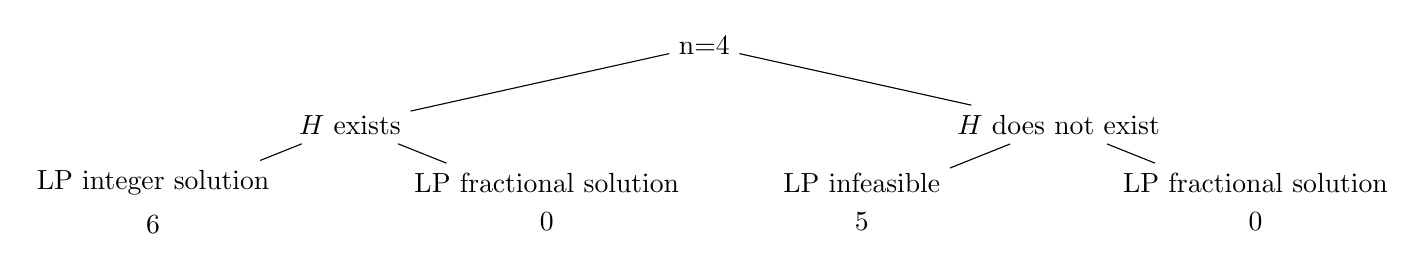
\begin{tikzpicture}[level distance=1cm,
  level 1/.style={sibling distance=9cm},
  level 2/.style={sibling distance=5cm}]
  \node {n=4}
    child { node {$H$ exists}
      child { node {$\underset{\raisebox{-0.8em}{6}}{\text{LP integer solution}}$} }
      child { node {$\underset{\raisebox{-0.8em}{0}}{\text{LP fractional solution}}$} }
    }
    child { node {$H$ does not exist}
      child { node {$\underset{\raisebox{-0.8em}{5}}{\text{LP infeasible}}$} }
      child { node {$\underset{\raisebox{-0.8em}{0}}{\text{LP fractional solution}}$} }
    };
\end{tikzpicture}

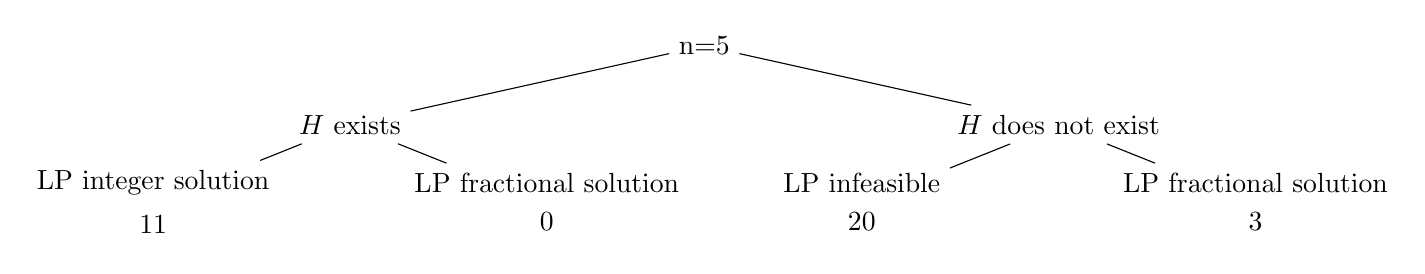
\begin{tikzpicture}[level distance=1cm,
  level 1/.style={sibling distance=9cm},
  level 2/.style={sibling distance=5cm}]
  \node {n=5}
    child { node {$H$ exists}
      child { node {$\underset{\raisebox{-0.8em}{11}}{\text{LP integer solution}}$} }
      child { node {$\underset{\raisebox{-0.8em}{0}}{\text{LP fractional solution}}$} }
    }
    child { node {$H$ does not exist}
      child { node {$\underset{\raisebox{-0.8em}{20}}{\text{LP infeasible}}$} }
      child { node {$\underset{\raisebox{-0.8em}{3}}{\text{LP fractional solution}}$} }
    };
\end{tikzpicture}

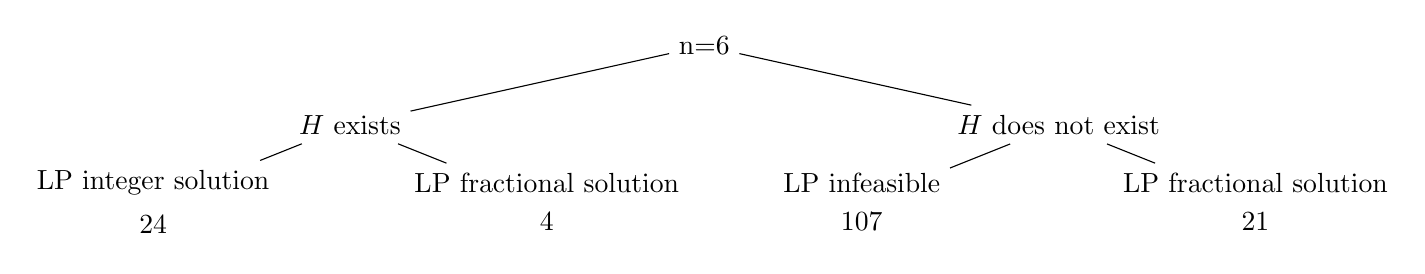
\begin{tikzpicture}[level distance=1cm,
  level 1/.style={sibling distance=9cm},
  level 2/.style={sibling distance=5cm}]
  \node {n=6}
    child { node {$H$ exists}
      child { node {$\underset{\raisebox{-0.8em}{24}}{\text{LP integer solution}}$} }
      child { node {$\underset{\raisebox{-0.8em}{4}}{\text{LP fractional solution}}$} }
    }
    child { node {$H$ does not exist}
      child { node {$\underset{\raisebox{-0.8em}{107}}{\text{LP infeasible}}$} }
      child { node {$\underset{\raisebox{-0.8em}{21}}{\text{LP fractional solution}}$} }
    };
\end{tikzpicture}

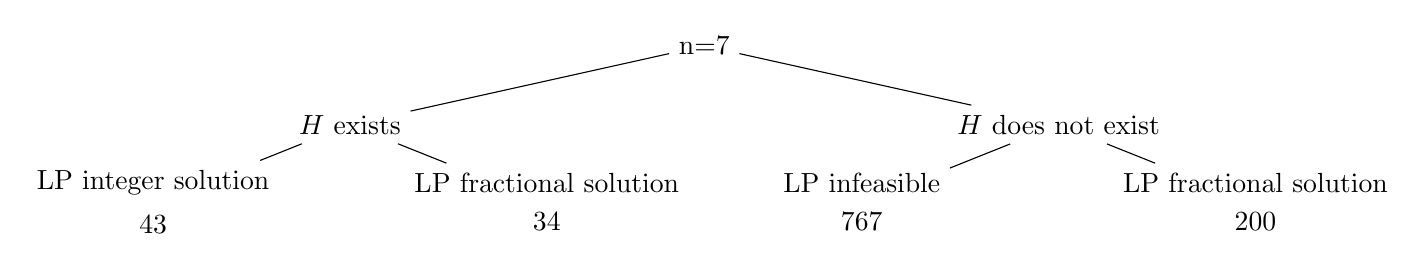
\begin{tikzpicture}[level distance=1cm,
  level 1/.style={sibling distance=9cm},
  level 2/.style={sibling distance=5cm}]
  \node {n=7}
    child { node {$H$ exists}
      child { node {$\underset{\raisebox{-0.8em}{43}}{\text{LP integer solution}}$} }
      child { node {$\underset{\raisebox{-0.8em}{34}}{\text{LP fractional solution}}$} }
    }
    child { node {$H$ does not exist}
      child { node {$\underset{\raisebox{-0.8em}{767}}{\text{LP infeasible}}$} }
      child { node {$\underset{\raisebox{-0.8em}{200}}{\text{LP fractional solution}}$} }
    };
\end{tikzpicture}

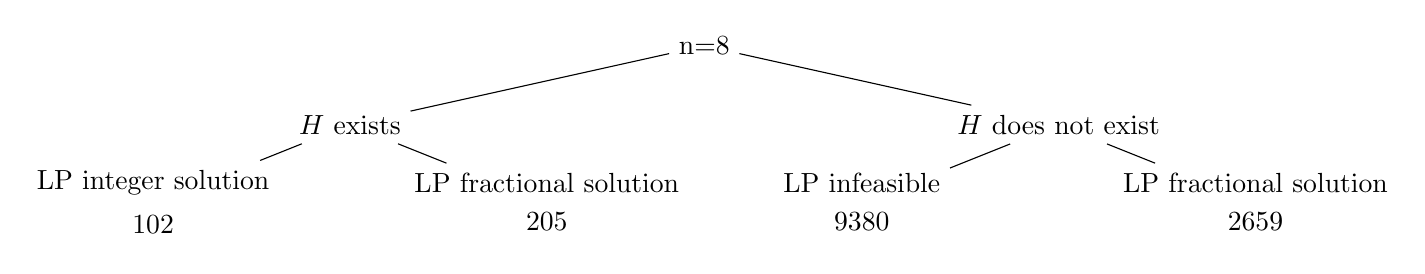
\begin{tikzpicture}[level distance=1cm,
  level 1/.style={sibling distance=9cm},
  level 2/.style={sibling distance=5cm}]
  \node {n=8}
    child { node {$H$ exists}
      child { node {$\underset{\raisebox{-0.8em}{102}}{\text{LP integer solution}}$} }
      child { node {$\underset{\raisebox{-0.8em}{205}}{\text{LP fractional solution}}$} }
    }
    child { node {$H$ does not exist}
      child { node {$\underset{\raisebox{-0.8em}{9380}}{\text{LP infeasible}}$} }
      child { node {$\underset{\raisebox{-0.8em}{2659}}{\text{LP fractional solution}}$} }
    };
\end{tikzpicture}

\caption{LP outcomes for different values of $n$ on the linear program with max objective function.}
\footnotemark
\label{fig:max_objective_function_diagram}
\end{figure}

\footnotetext{The LP integer 
solution sequence $3, 6, 11, 22, 42, 102, \dots$ is very similar to the 
number of distinct characteristic polynomials of tress with $n$ nodes - \href{https://oeis.org/A226594}{A226594}.}

\newpage

\subsubsection{Singular Triangular Decomposition}
\begin{figure}[!htbp]
\centering

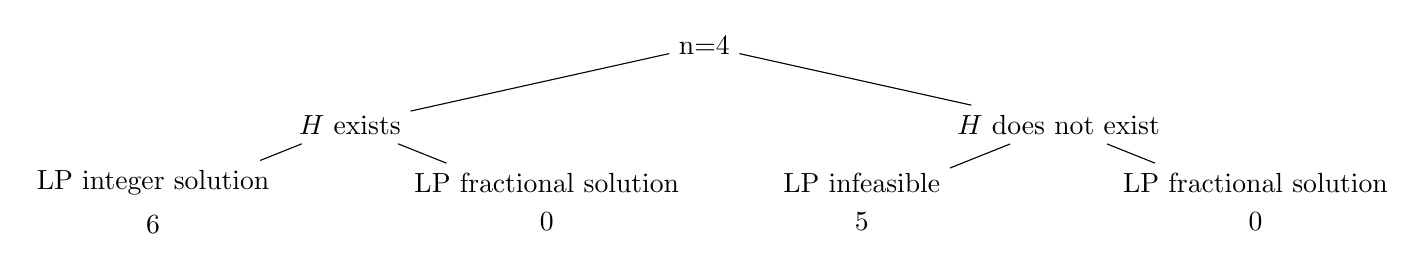
\begin{tikzpicture}[level distance=1cm,
  level 1/.style={sibling distance=9cm},
  level 2/.style={sibling distance=5cm}]
  \node {n=4}
    child { node {$H$ exists}
      child { node {$\underset{\raisebox{-0.8em}{6}}{\text{LP integer solution}}$} }
      child { node {$\underset{\raisebox{-0.8em}{0}}{\text{LP fractional solution}}$} }
    }
    child { node {$H$ does not exist}
      child { node {$\underset{\raisebox{-0.8em}{5}}{\text{LP infeasible}}$} }
      child { node {$\underset{\raisebox{-0.8em}{0}}{\text{LP fractional solution}}$} }
    };
\end{tikzpicture}

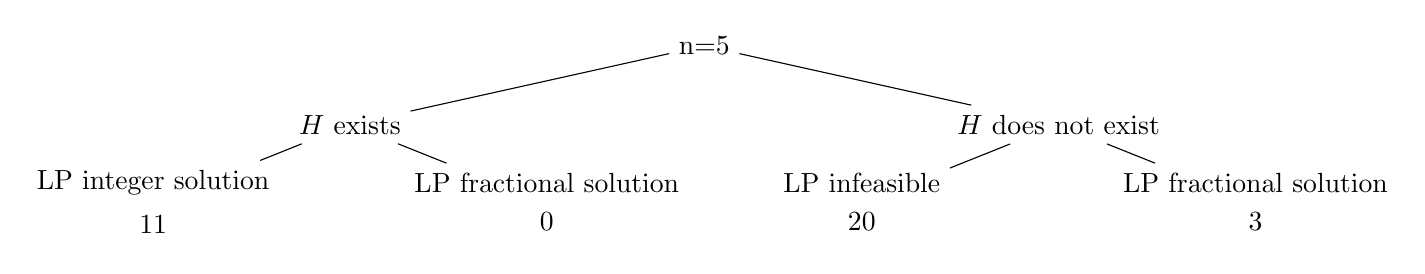
\begin{tikzpicture}[level distance=1cm,
  level 1/.style={sibling distance=9cm},
  level 2/.style={sibling distance=5cm}]
  \node {n=5}
    child { node {$H$ exists}
      child { node {$\underset{\raisebox{-0.8em}{11}}{\text{LP integer solution}}$} }
      child { node {$\underset{\raisebox{-0.8em}{0}}{\text{LP fractional solution}}$} }
    }
    child { node {$H$ does not exist}
      child { node {$\underset{\raisebox{-0.8em}{20}}{\text{LP infeasible}}$} }
      child { node {$\underset{\raisebox{-0.8em}{3}}{\text{LP fractional solution}}$} }
    };
\end{tikzpicture}

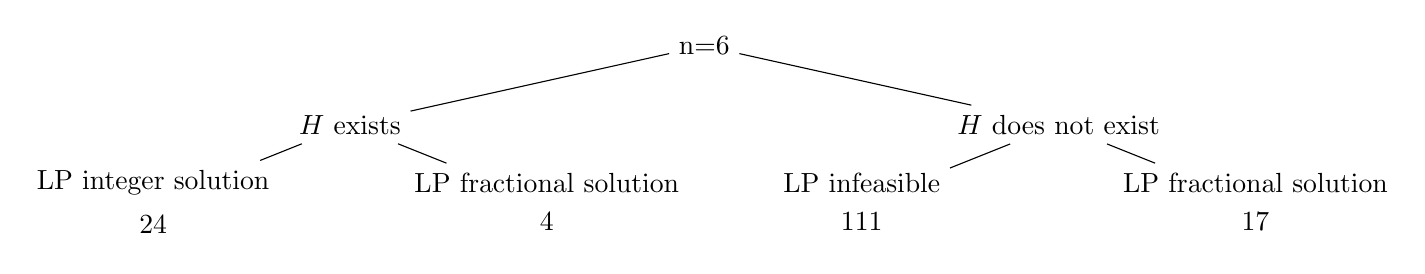
\begin{tikzpicture}[level distance=1cm,
  level 1/.style={sibling distance=9cm},
  level 2/.style={sibling distance=5cm}]
  \node {n=6}
    child { node {$H$ exists}
      child { node {$\underset{\raisebox{-0.8em}{24}}{\text{LP integer solution}}$} }
      child { node {$\underset{\raisebox{-0.8em}{4}}{\text{LP fractional solution}}$} }
    }
    child { node {$H$ does not exist}
      child { node {$\underset{\raisebox{-0.8em}{111}}{\text{LP infeasible}}$} }
      child { node {$\underset{\raisebox{-0.8em}{17}}{\text{LP fractional solution}}$} }
    };
\end{tikzpicture}

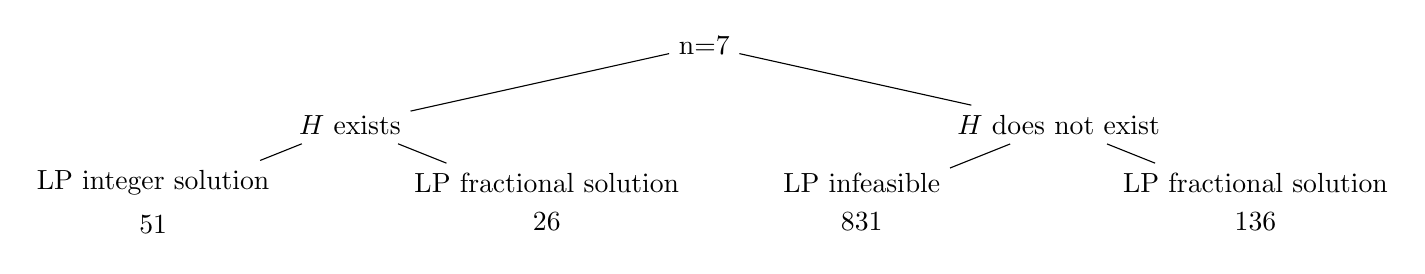
\begin{tikzpicture}[level distance=1cm,
  level 1/.style={sibling distance=9cm},
  level 2/.style={sibling distance=5cm}]
  \node {n=7}
    child { node {$H$ exists}
      child { node {$\underset{\raisebox{-0.8em}{51}}{\text{LP integer solution}}$} }
      child { node {$\underset{\raisebox{-0.8em}{26}}{\text{LP fractional solution}}$} }
    }
    child { node {$H$ does not exist}
      child { node {$\underset{\raisebox{-0.8em}{831}}{\text{LP infeasible}}$} }
      child { node {$\underset{\raisebox{-0.8em}{136}}{\text{LP fractional solution}}$} }
    };
\end{tikzpicture}

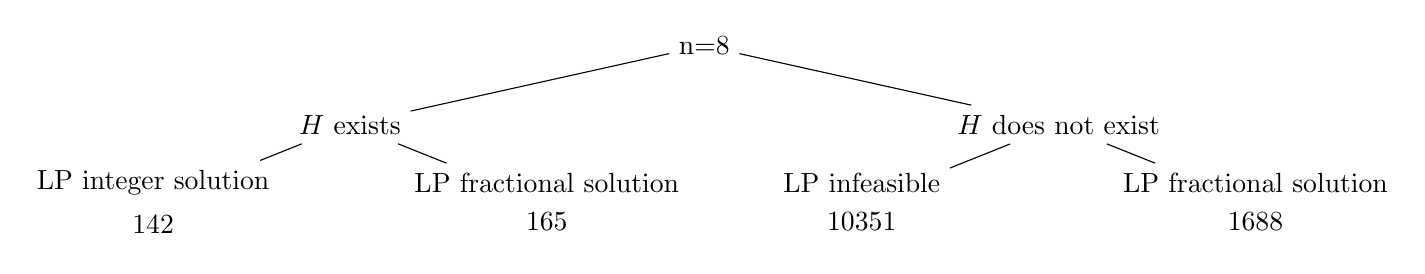
\begin{tikzpicture}[level distance=1cm,
  level 1/.style={sibling distance=9cm},
  level 2/.style={sibling distance=5cm}]
  \node {n=8}
    child { node {$H$ exists}
      child { node {$\underset{\raisebox{-0.8em}{142}}{\text{LP integer solution}}$} }
      child { node {$\underset{\raisebox{-0.8em}{165}}{\text{LP fractional solution}}$} }
    }
    child { node {$H$ does not exist}
      child { node {$\underset{\raisebox{-0.8em}{10351}}{\text{LP infeasible}}$} }
      child { node {$\underset{\raisebox{-0.8em}{1688}}{\text{LP fractional solution}}$} }
    };
\end{tikzpicture}

\caption{LP outcomes for different values of $n$ on the linear program with max objective function 
and singular triangular decomposition.}
\label{fig:singular_triangular_decomposition_diagram}
\end{figure}

\newpage

\begin{figure}[!htbp]
\centering

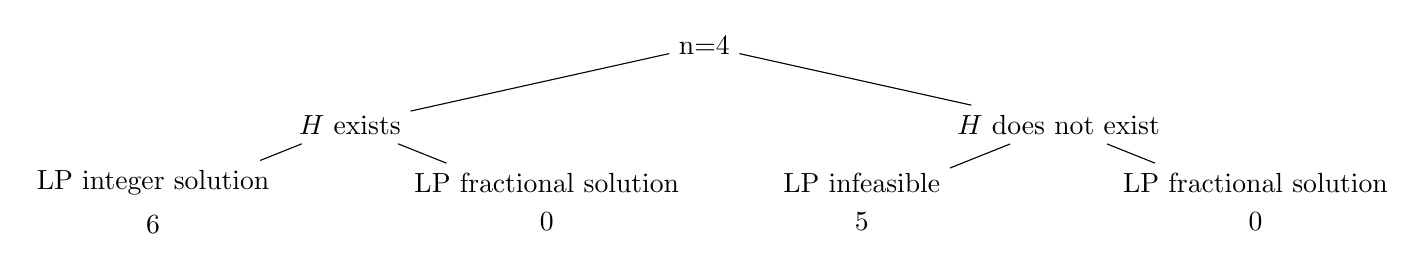
\begin{tikzpicture}[level distance=1cm,
  level 1/.style={sibling distance=9cm},
  level 2/.style={sibling distance=5cm}]
  \node {n=4}
    child { node {$H$ exists}
      child { node {$\underset{\raisebox{-0.8em}{6}}{\text{LP integer solution}}$} }
      child { node {$\underset{\raisebox{-0.8em}{0}}{\text{LP fractional solution}}$} }
    }
    child { node {$H$ does not exist}
      child { node {$\underset{\raisebox{-0.8em}{5}}{\text{LP infeasible}}$} }
      child { node {$\underset{\raisebox{-0.8em}{0}}{\text{LP fractional solution}}$} }
    };
\end{tikzpicture}

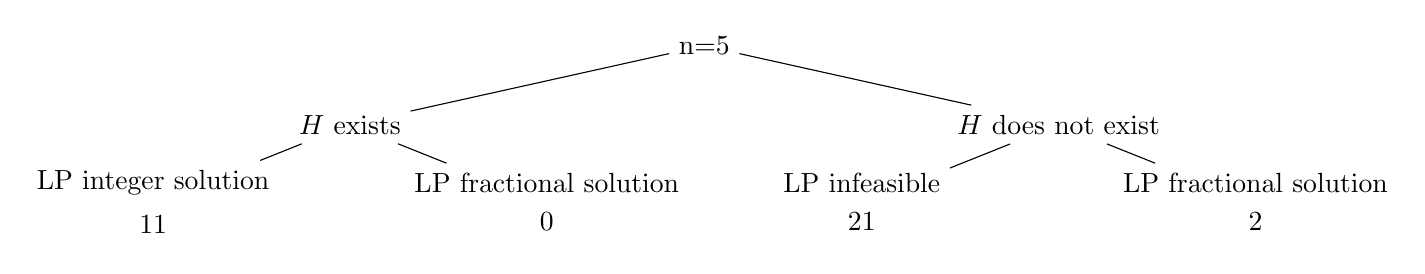
\begin{tikzpicture}[level distance=1cm,
  level 1/.style={sibling distance=9cm},
  level 2/.style={sibling distance=5cm}]
  \node {n=5}
    child { node {$H$ exists}
      child { node {$\underset{\raisebox{-0.8em}{11}}{\text{LP integer solution}}$} }
      child { node {$\underset{\raisebox{-0.8em}{0}}{\text{LP fractional solution}}$} }
    }
    child { node {$H$ does not exist}
      child { node {$\underset{\raisebox{-0.8em}{21}}{\text{LP infeasible}}$} }
      child { node {$\underset{\raisebox{-0.8em}{2}}{\text{LP fractional solution}}$} }
    };
\end{tikzpicture}

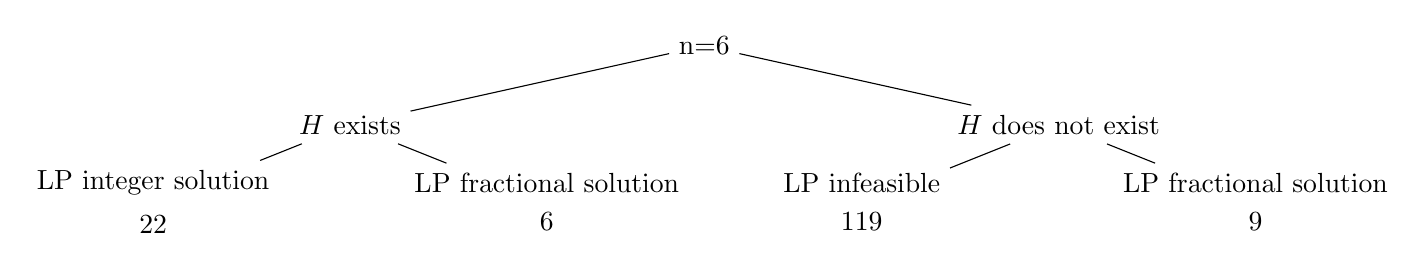
\begin{tikzpicture}[level distance=1cm,
  level 1/.style={sibling distance=9cm},
  level 2/.style={sibling distance=5cm}]
  \node {n=6}
    child { node {$H$ exists}
      child { node {$\underset{\raisebox{-0.8em}{22}}{\text{LP integer solution}}$} }
      child { node {$\underset{\raisebox{-0.8em}{6}}{\text{LP fractional solution}}$} }
    }
    child { node {$H$ does not exist}
      child { node {$\underset{\raisebox{-0.8em}{119}}{\text{LP infeasible}}$} }
      child { node {$\underset{\raisebox{-0.8em}{9}}{\text{LP fractional solution}}$} }
    };
\end{tikzpicture}

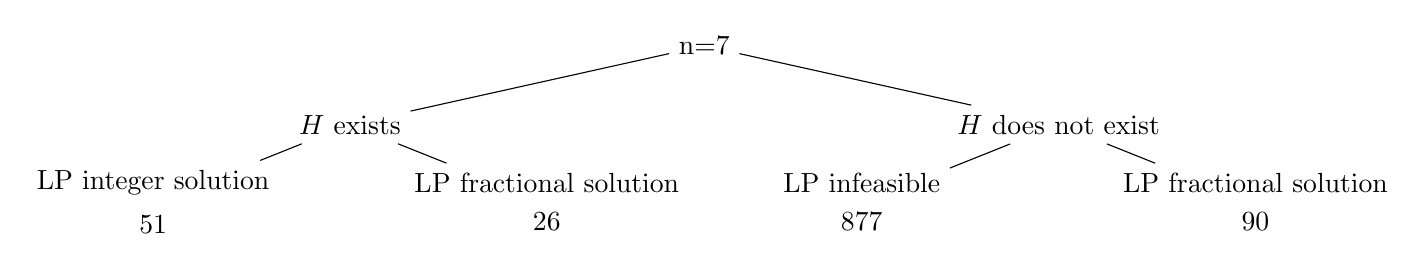
\begin{tikzpicture}[level distance=1cm,
  level 1/.style={sibling distance=9cm},
  level 2/.style={sibling distance=5cm}]
  \node {n=7}
    child { node {$H$ exists}
      child { node {$\underset{\raisebox{-0.8em}{51}}{\text{LP integer solution}}$} }
      child { node {$\underset{\raisebox{-0.8em}{26}}{\text{LP fractional solution}}$} }
    }
    child { node {$H$ does not exist}
      child { node {$\underset{\raisebox{-0.8em}{877}}{\text{LP infeasible}}$} }
      child { node {$\underset{\raisebox{-0.8em}{90}}{\text{LP fractional solution}}$} }
    };
\end{tikzpicture}

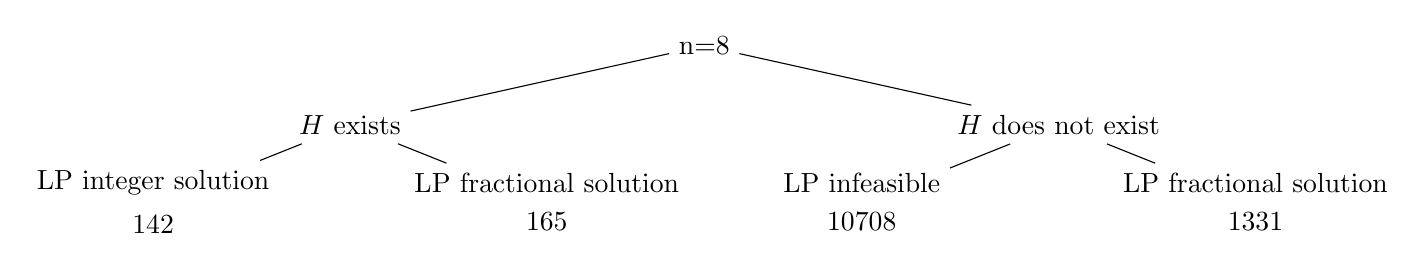
\begin{tikzpicture}[level distance=1cm,
  level 1/.style={sibling distance=9cm},
  level 2/.style={sibling distance=5cm}]
  \node {n=8}
    child { node {$H$ exists}
      child { node {$\underset{\raisebox{-0.8em}{142}}{\text{LP integer solution}}$} }
      child { node {$\underset{\raisebox{-0.8em}{165}}{\text{LP fractional solution}}$} }
    }
    child { node {$H$ does not exist}
      child { node {$\underset{\raisebox{-0.8em}{10708}}{\text{LP infeasible}}$} }
      child { node {$\underset{\raisebox{-0.8em}{1331}}{\text{LP fractional solution}}$} }
    };
\end{tikzpicture}

\caption{LP outcomes for different values of $n$ on the linear program with max objective function 
and singular triangular decomposition with recursion for tie-breaking.}
\label{fig:recursive_singular_triangular_decomposition_diagram}
\end{figure}

\newpage

\subsubsection{Rounding}

\begin{figure}[!htbp]
\centering

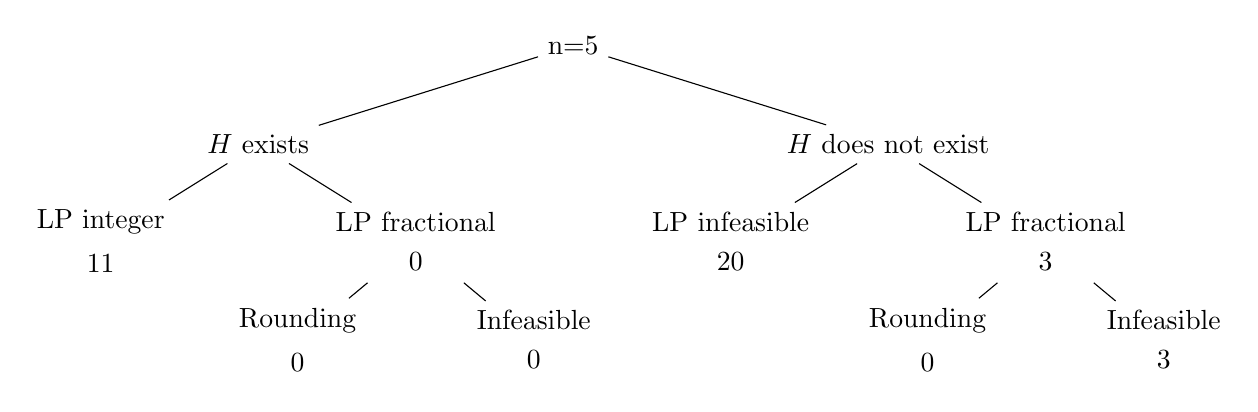
\begin{tikzpicture}[level distance=1.25cm,
  level 1/.style={sibling distance=8cm},
  level 2/.style={sibling distance=4cm},
  level 3/.style={sibling distance=3cm}]
  \node {n=5}
    child { node {$H$ exists}
      child { node {$\underset{\raisebox{-0.8em}{11}}{\text{LP integer}}$} }
      child { node {$\underset{\raisebox{-0.8em}{0}}{\text{LP fractional}}$} 
        child { node {$\underset{\raisebox{-0.8em}{0}}{\text{Rounding}}$}  }
        child { node {$\underset{\raisebox{-0.8em}{0}}{\text{Infeasible}}$}  }
      }
    }
    child { node {$H$ does not exist}
      child { node {$\underset{\raisebox{-0.8em}{20}}{\text{LP infeasible}}$} }
      child { node {$\underset{\raisebox{-0.8em}{3}}{\text{LP fractional}}$} 
        child { node {$\underset{\raisebox{-0.8em}{0}}{\text{Rounding}}$}  }
        child { node {$\underset{\raisebox{-0.8em}{3}}{\text{Infeasible}}$}  }
      }
    };
\end{tikzpicture}

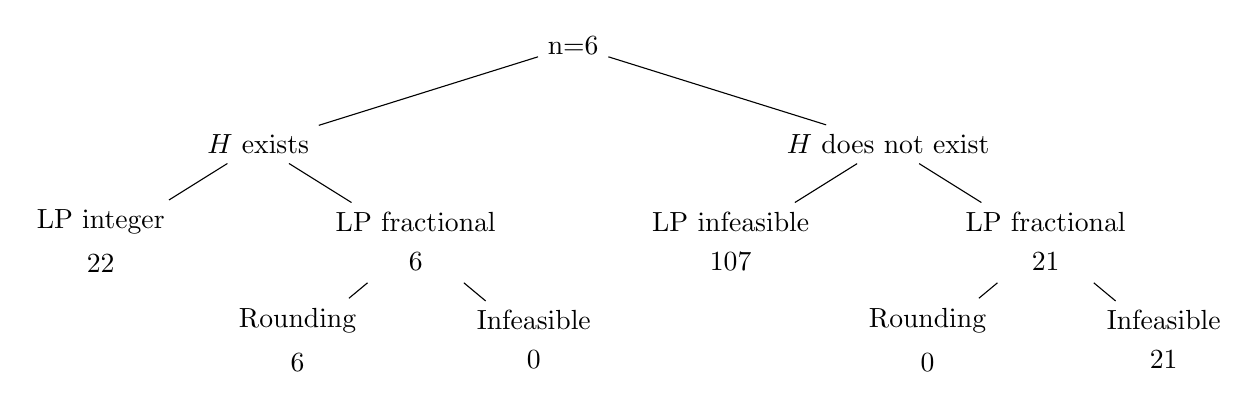
\begin{tikzpicture}[level distance=1.25cm,
  level 1/.style={sibling distance=8cm},
  level 2/.style={sibling distance=4cm},
  level 3/.style={sibling distance=3cm}]
  \node {n=6}
    child { node {$H$ exists}
      child { node {$\underset{\raisebox{-0.8em}{22}}{\text{LP integer}}$} }
      child { node {$\underset{\raisebox{-0.8em}{6}}{\text{LP fractional}}$} 
        child { node {$\underset{\raisebox{-0.8em}{6}}{\text{Rounding}}$}  }
        child { node {$\underset{\raisebox{-0.8em}{0}}{\text{Infeasible}}$}  }
      }
    }
    child { node {$H$ does not exist}
      child { node {$\underset{\raisebox{-0.8em}{107}}{\text{LP infeasible}}$} }
      child { node {$\underset{\raisebox{-0.8em}{21}}{\text{LP fractional}}$} 
        child { node {$\underset{\raisebox{-0.8em}{0}}{\text{Rounding}}$}  }
        child { node {$\underset{\raisebox{-0.8em}{21}}{\text{Infeasible}}$}  }
      }
    };
\end{tikzpicture}

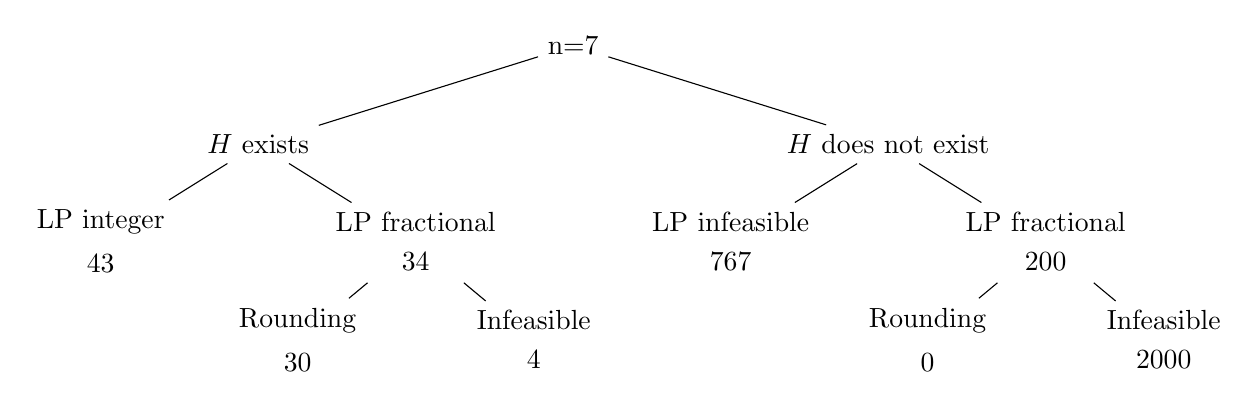
\begin{tikzpicture}[level distance=1.25cm,
  level 1/.style={sibling distance=8cm},
  level 2/.style={sibling distance=4cm},
  level 3/.style={sibling distance=3cm}]
  \node {n=7}
    child { node {$H$ exists}
      child { node {$\underset{\raisebox{-0.8em}{43}}{\text{LP integer}}$} }
      child { node {$\underset{\raisebox{-0.8em}{34}}{\text{LP fractional}}$} 
        child { node {$\underset{\raisebox{-0.8em}{30}}{\text{Rounding}}$}  }
        child { node {$\underset{\raisebox{-0.8em}{4}}{\text{Infeasible}}$}  }
      }
    }
    child { node {$H$ does not exist}
      child { node {$\underset{\raisebox{-0.8em}{767}}{\text{LP infeasible}}$} }
      child { node {$\underset{\raisebox{-0.8em}{200}}{\text{LP fractional}}$} 
        child { node {$\underset{\raisebox{-0.8em}{0}}{\text{Rounding}}$}  }
        child { node {$\underset{\raisebox{-0.8em}{2000}}{\text{Infeasible}}$}  }
      }
    };
\end{tikzpicture}

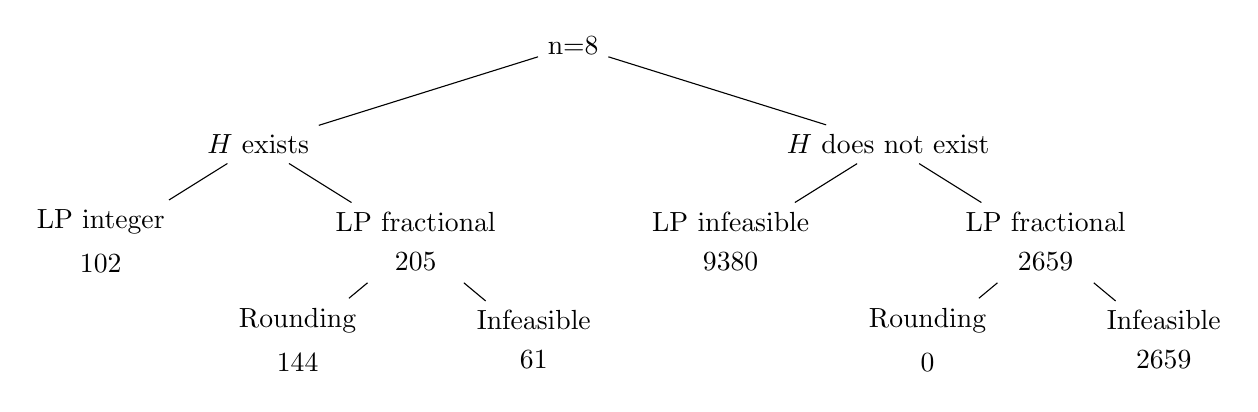
\begin{tikzpicture}[level distance=1.25cm,
  level 1/.style={sibling distance=8cm},
  level 2/.style={sibling distance=4cm},
  level 3/.style={sibling distance=3cm}]
  \node {n=8}
    child { node {$H$ exists}
      child { node {$\underset{\raisebox{-0.8em}{102}}{\text{LP integer}}$} }
      child { node {$\underset{\raisebox{-0.8em}{205}}{\text{LP fractional}}$} 
        child { node {$\underset{\raisebox{-0.8em}{144}}{\text{Rounding}}$}  }
        child { node {$\underset{\raisebox{-0.8em}{61}}{\text{Infeasible}}$}  }
      }
    }
    child { node {$H$ does not exist}
      child { node {$\underset{\raisebox{-0.8em}{9380}}{\text{LP infeasible}}$} }
      child { node {$\underset{\raisebox{-0.8em}{2659}}{\text{LP fractional}}$} 
        child { node {$\underset{\raisebox{-0.8em}{0}}{\text{Rounding}}$}  }
        child { node {$\underset{\raisebox{-0.8em}{2659}}{\text{Infeasible}}$}  }
      }
    };
\end{tikzpicture}

\caption{LP outcomes for different values of $n$ on the linear program with max objective function 
and using rounding for fractional solutions.}
\label{fig:rounding_max_objective_function_diagram}
\end{figure}

\newpage

\begin{figure}[!htbp]
\centering

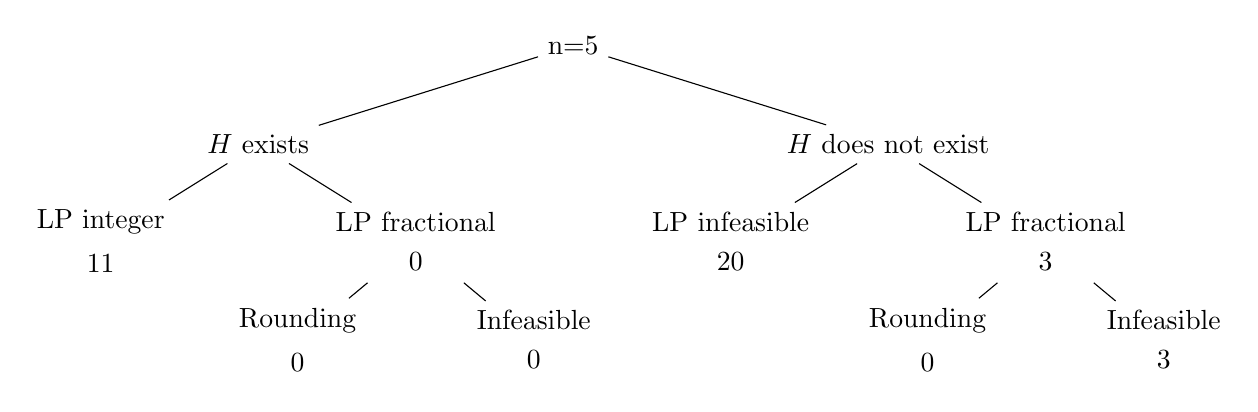
\begin{tikzpicture}[level distance=1.25cm,
  level 1/.style={sibling distance=8cm},
  level 2/.style={sibling distance=4cm},
  level 3/.style={sibling distance=3cm}]
  \node {n=5}
    child { node {$H$ exists}
      child { node {$\underset{\raisebox{-0.8em}{11}}{\text{LP integer}}$} }
      child { node {$\underset{\raisebox{-0.8em}{0}}{\text{LP fractional}}$} 
        child { node {$\underset{\raisebox{-0.8em}{0}}{\text{Rounding}}$}  }
        child { node {$\underset{\raisebox{-0.8em}{0}}{\text{Infeasible}}$}  }
      }
    }
    child { node {$H$ does not exist}
      child { node {$\underset{\raisebox{-0.8em}{20}}{\text{LP infeasible}}$} }
      child { node {$\underset{\raisebox{-0.8em}{3}}{\text{LP fractional}}$} 
        child { node {$\underset{\raisebox{-0.8em}{0}}{\text{Rounding}}$}  }
        child { node {$\underset{\raisebox{-0.8em}{3}}{\text{Infeasible}}$}  }
      }
    };
\end{tikzpicture}

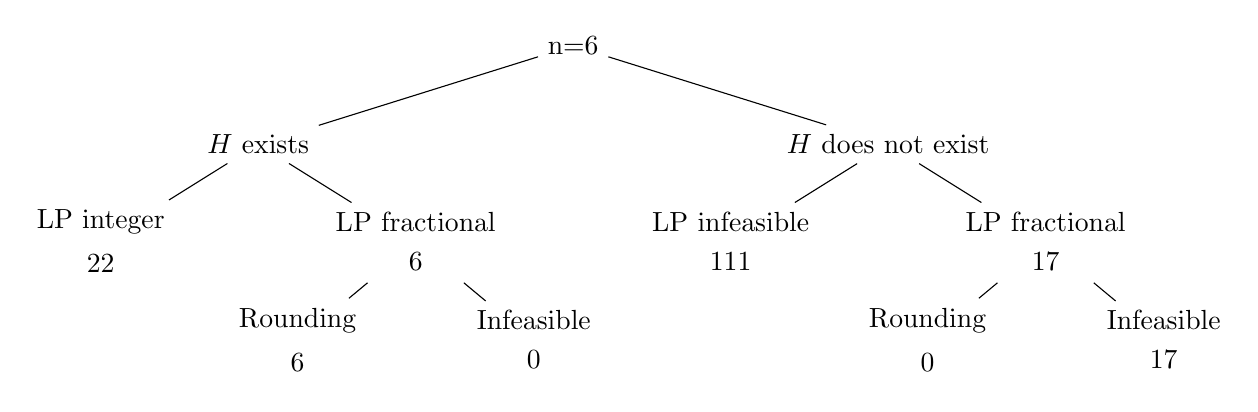
\begin{tikzpicture}[level distance=1.25cm,
  level 1/.style={sibling distance=8cm},
  level 2/.style={sibling distance=4cm},
  level 3/.style={sibling distance=3cm}]
  \node {n=6}
    child { node {$H$ exists}
      child { node {$\underset{\raisebox{-0.8em}{22}}{\text{LP integer}}$} }
      child { node {$\underset{\raisebox{-0.8em}{6}}{\text{LP fractional}}$} 
        child { node {$\underset{\raisebox{-0.8em}{6}}{\text{Rounding}}$}  }
        child { node {$\underset{\raisebox{-0.8em}{0}}{\text{Infeasible}}$}  }
      }
    }
    child { node {$H$ does not exist}
      child { node {$\underset{\raisebox{-0.8em}{111}}{\text{LP infeasible}}$} }
      child { node {$\underset{\raisebox{-0.8em}{17}}{\text{LP fractional}}$} 
        child { node {$\underset{\raisebox{-0.8em}{0}}{\text{Rounding}}$}  }
        child { node {$\underset{\raisebox{-0.8em}{17}}{\text{Infeasible}}$}  }
      }
    };
\end{tikzpicture}

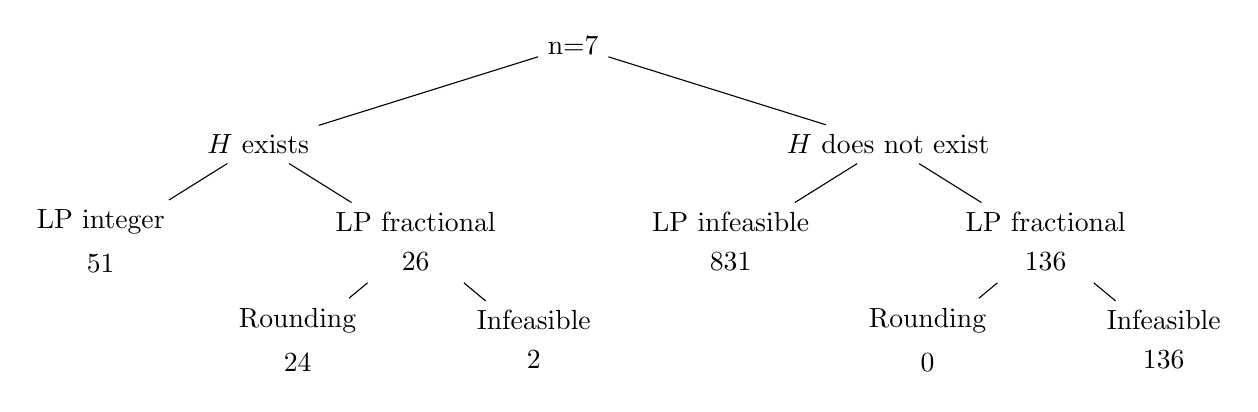
\begin{tikzpicture}[level distance=1.25cm,
  level 1/.style={sibling distance=8cm},
  level 2/.style={sibling distance=4cm},
  level 3/.style={sibling distance=3cm}]
  \node {n=7}
    child { node {$H$ exists}
      child { node {$\underset{\raisebox{-0.8em}{51}}{\text{LP integer}}$} }
      child { node {$\underset{\raisebox{-0.8em}{26}}{\text{LP fractional}}$} 
        child { node {$\underset{\raisebox{-0.8em}{24}}{\text{Rounding}}$}  }
        child { node {$\underset{\raisebox{-0.8em}{2}}{\text{Infeasible}}$}  }
      }
    }
    child { node {$H$ does not exist}
      child { node {$\underset{\raisebox{-0.8em}{831}}{\text{LP infeasible}}$} }
      child { node {$\underset{\raisebox{-0.8em}{136}}{\text{LP fractional}}$} 
        child { node {$\underset{\raisebox{-0.8em}{0}}{\text{Rounding}}$}  }
        child { node {$\underset{\raisebox{-0.8em}{136}}{\text{Infeasible}}$}  }
      }
    };
\end{tikzpicture}

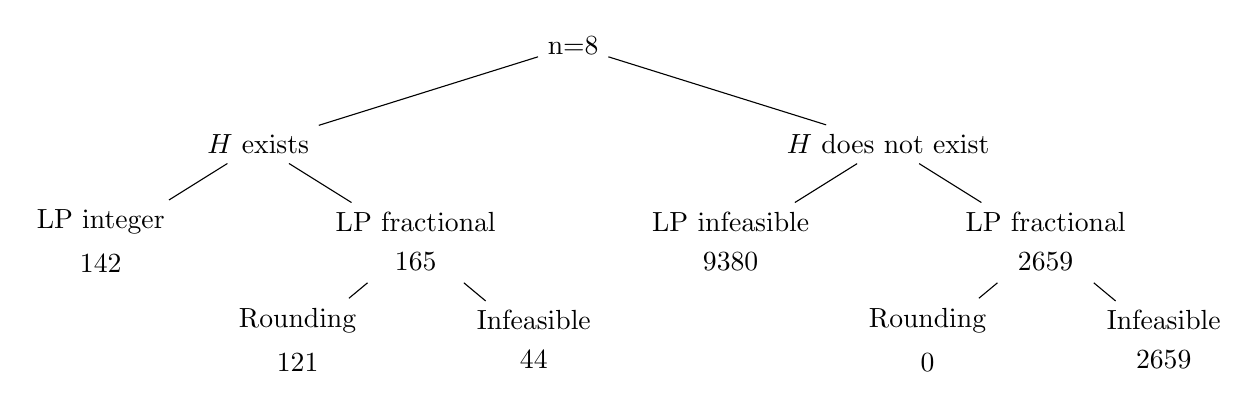
\begin{tikzpicture}[level distance=1.25cm,
  level 1/.style={sibling distance=8cm},
  level 2/.style={sibling distance=4cm},
  level 3/.style={sibling distance=3cm}]
  \node {n=8}
    child { node {$H$ exists}
      child { node {$\underset{\raisebox{-0.8em}{142}}{\text{LP integer}}$} }
      child { node {$\underset{\raisebox{-0.8em}{165}}{\text{LP fractional}}$} 
        child { node {$\underset{\raisebox{-0.8em}{121}}{\text{Rounding}}$}  }
        child { node {$\underset{\raisebox{-0.8em}{44}}{\text{Infeasible}}$}  }
      }
    }
    child { node {$H$ does not exist}
      child { node {$\underset{\raisebox{-0.8em}{9380}}{\text{LP infeasible}}$} }
      child { node {$\underset{\raisebox{-0.8em}{2659}}{\text{LP fractional}}$} 
        child { node {$\underset{\raisebox{-0.8em}{0}}{\text{Rounding}}$}  }
        child { node {$\underset{\raisebox{-0.8em}{2659}}{\text{Infeasible}}$}  }
      }
    };
\end{tikzpicture}

\caption{LP outcomes for different values of $n$ on the linear program with max objective function, singular 
triangular decomposition and using rounding for fractional solutions.}
\label{fig:rounding_triangular_max_objective_function_diagram}
\end{figure}

\newpage

\subsection{Dual Program}

\begin{figure}[!htbp]
\centering

\begin{tikzpicture}[
  level distance=1.25cm,
  level 1/.style={sibling distance=9cm},
  level 2/.style={sibling distance=4.1cm},
  level 3/.style={sibling distance=2.1cm},
  every node/.style={align=center, font=\tiny}
]

\node {n = 6}
  child { node {$H$ exists}
    child { node {$\underset{\raisebox{-0.8em}{}}{\text{Primal integer}}$} 
      child { node {$\underset{\raisebox{-0.8em}{}}{\text{Dual feasible}}$}  }
      child { node {$\underset{\raisebox{-0.8em}{}}{\text{Dual infeasible}}$}  }
    }
    child { node {$\underset{\raisebox{-0.8em}{}}{\text{Primal fractional}}$} 
      child { node {$\underset{\raisebox{-0.8em}{}}{\text{Dual feasible}}$}  }
      child { node {$\underset{\raisebox{-0.8em}{}}{\text{Dual unbounded}}$}  }
    }
  }
  child { node {$H$ does not exist}
    child { node {$\underset{\raisebox{-0.8em}{}}{\text{Primal infeasible}}$} 
      child { node {$\underset{\raisebox{-0.8em}{}}{\text{Dual feasible }}$}  }
      child { node {$\underset{\raisebox{-0.8em}{}}{\text{Dual infeasible}}$}  }
    }
    child { node {$\underset{\raisebox{-0.8em}{}}{\text{Primal fractional}}$} 
      child { node {$\underset{\raisebox{-0.8em}{}}{\text{Dual feasible }}$}  }
      child { node {$\underset{\raisebox{-0.8em}{}}{\text{Dual infeasible}}$}  }
    }
  };

\end{tikzpicture}

\caption{LP outcomes for different values of $n$ on the dual linear program.}
\label{fig:duak_objective_function_diagram}
\end{figure}

\newpage

\printbibliography

\end{document}
